\documentclass[tikz,border=5mm]{standalone}
\usetikzlibrary{arrows.meta}
\usepackage{amsmath}

\begin{document}
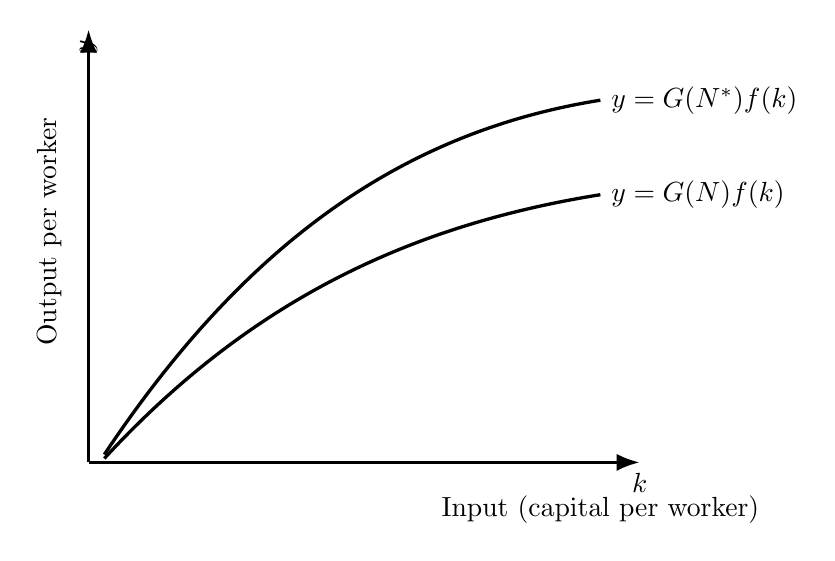
\begin{tikzpicture}[scale=1]

    % Define the coordinate system
    \coordinate (O) at (0,0);
    
    % Draw axes
    \draw[-Latex, very thick] (0,0) -- (7,0) node[below] {$k$};
    \draw[-Latex, very thick] (0,0) -- (0,5.5) node[left, rotate=90, anchor=east] {$y$};
    
    % Add axis labels
    \node[below] at (6.5,-0.3) {Input (capital per worker)};
    \node[left, rotate=90, anchor=east] at (-0.5,4.5) {Output per worker};
    
    % Draw the upper production function curve
    \draw[very thick, smooth] (0.2,0.1) .. controls (2,2.8) and (4,4.2) .. (6.5,4.6) node[right] {$y=G(N^*)f(k)$};
    
    % Draw the lower production function curve
    \draw[very thick, smooth] (0.2,0.05) .. controls (2,2) and (4,3) .. (6.5,3.4) node[right] {$y=G(N)f(k)$};
    
\end{tikzpicture}
\end{document}